\documentclass{article}
\usepackage[utf8]{inputenc}
\usepackage[english]{babel}
\usepackage{amsmath}
\usepackage{amsthm}
\usepackage{amssymb}
\usepackage{enumitem}
\usepackage{underscore}

\usepackage{tikz}
\usetikzlibrary{positioning, calc, shapes.geometric, shapes.multipart, 
	shapes, arrows.meta, arrows, 
	decorations.markings, external, trees}

\tikzstyle{Arrow} = [
	thick,
	decoration={
		markings,
		mark=at position 1 with {
			\arrow[thick]{latex}
			}
		},
	shorten >= 3pt, preaction = {decorate}
	]

\begin{document}

\section*{Problem 1}
\begin{proof}
We want to show that 
	\begin{equation*} 
		Pr(\alpha_1, ..., \alpha_n) = \prod_{i=1}^n Pr(\alpha_i | \alpha_{i+1}, ..., \alpha_{n}, \beta)
	\end{equation*}
We will induct on n. \\
First we assert our base cases: \\
\indent We can observe trivially that the identity holds for n = 0 and n = 1. \\
\indent For n=2, we can observe by Bayes' Conditioning Rule that \begin{equation*}
	 Pr(\alpha_1, \alpha_2 | \beta) = Pr(\alpha_1 | \alpha_2, \beta) Pr(\alpha_2 | \beta) \end{equation*}
We will now prove the inductive case: \\
\indent Assume that 
	\begin{equation*} 
		Pr(\alpha_1, ..., \alpha_n | \beta) = \prod_{i=1}^n Pr(\alpha_i | \alpha_{i+1}, ..., \alpha_{n}, \beta)
	\end{equation*}
	Then by Bayes' Conditioning Rule,
	 \begin{align*}
		Pr(\alpha_1, ..., &\alpha_{n+1} | \beta) \\
			\indent &= Pr(\alpha_{n+1} | \alpha_1, ..., \alpha_n, \beta) 
				Pr(\alpha_1 | \alpha_2, ..., \alpha_n, \beta) ... Pr(\alpha_n | \beta) \\
			&= \frac {Pr(\alpha_{n+1}, \alpha_1 | \alpha_2, ..., \alpha_n, \beta)} 
				     {Pr(\alpha_1 | \alpha_2, ..., \alpha_n, \beta)}
				\biggr( Pr(\alpha_1 | \alpha_2, ..., \alpha_n, \beta) ... Pr(\alpha_n | \beta) \biggr)\\
			&= \frac {Pr(\alpha_1 | \alpha_2, ..., \alpha_{n+1}, \beta) 
					Pr(\alpha_{n+1} | \alpha_2, ..., \alpha_n, \beta)}
				     {Pr(\alpha_1 | \alpha_2, ..., \alpha_n, \beta)}
				\biggr( Pr(\alpha_1 | \alpha_2, ..., \alpha_n, \beta) ... Pr(\alpha_n | \beta) \biggr)\\
			&= Pr(\alpha_1 | \alpha_2, ..., \alpha_{n+1}, \beta) Pr(\alpha_{n+1} | \alpha_2, ..., \alpha_n, \beta)
				\biggr( Pr(\alpha_2 | \alpha_3, ..., \alpha_n, \beta) ... Pr(\alpha_1, ..., \alpha_n | \beta) \biggr)\\
			&= Pr(\alpha_1 | \alpha_2, ..., \alpha_n, \beta)
				Pr(\alpha_2 | \alpha_3, ..., \alpha_n, \beta)
				Pr(\alpha_{n+1} | \alpha_3, ..., \alpha_n, \beta)
				\biggr(Pr(\alpha_3 | \alpha_4, ..., \alpha_n, \beta) ... Pr(\alpha_n | \beta) \biggr)
	\end{align*}
	We can extrapolate this out to see
	\begin{align*}
		Pr(\alpha_1, ..., \alpha_{n+1} | \beta) 
			&= \frac {Pr(\alpha_{n+1} | \beta)}  {Pr(\alpha_n |\beta)}
				\biggr( Pr(\alpha_1 | \alpha_2, ..., \alpha_{n+1}, \beta) ... Pr(\alpha_{n-1} | \alpha_n, \beta) \biggr)
				 Pr( \alpha_n | \beta) \\
			&= Pr(\alpha_1 | \alpha_2, ..., \alpha_{n+1}, \beta) ... Pr(\alpha_{n+1} | \beta) \\
			&= \prod_{i=1}^{n+1} Pr(\alpha_i | \alpha_{i+1}, ..., \alpha_{n+1}, \beta)
	\end{align*}\end{proof}
\clearpage

\section*{Problem 2}
We use the following variables: \\
\indent o denotes the presence of oil. \\
\indent g denotes the presence of natural gas. \\
\indent t denotes a positive geographic test.\\
Then \begin{align*}Pr(o | t)
	&= \frac {Pr(o)} {Pr(t)} Pr(t | o) \\
	&= \frac {Pr(o) Pr(t | o)} {Pr(t | o) Pr (o) + P(t | g) Pr(g) + Pr(t | \bar o, \bar g) P(\bar o, \bar g)} \\
	&= \frac {(0.5) (0.9)} {(0.9) (0.5) + (0.3) (0.2) + (0.1) (0.3)} = 0.833
\end{align*}
\clearpage

\section*{Problem 3}
We let a positive literal denote a heads on a flip, and a negative denote a tails.\\
We also let $H_n$ denote a heads on the n'th coin flip.\\
\begin{center}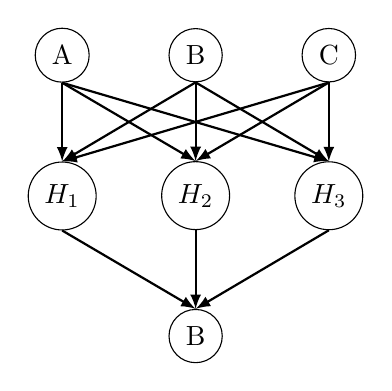
\begin{tikzpicture}
	%nodes:
		\node [circle, draw] (1) {A};
		\node [circle, draw, right =of 1] (2) {B};
		\node [circle, draw, right =of 2] (3) {C};
		\node [circle, draw, below =of 1] (4) {$H_1$};
		\node [circle, draw, below =of 2] (5) {$H_2$};
		\node [circle, draw, below =of 3] (6) {$H_3$};
		\node [circle, draw, below =of 5] (7) {B};
	%edges:
		\draw[Arrow] (1.south) -- (4.north);
		\draw[Arrow] (1.south) -- (5.north);
		\draw[Arrow] (1.south) -- (6.north);
		\draw[Arrow] (2.south) -- (4.north);
		\draw[Arrow] (2.south) -- (5.north);
		\draw[Arrow] (2.south) -- (6.north);
		\draw[Arrow] (3.south) -- (4.north);
		\draw[Arrow] (3.south) -- (5.north);
		\draw[Arrow] (3.south) -- (6.north);
		\draw[Arrow] (4.south) -- (7.north);
		\draw[Arrow] (5.south) -- (7.north);
		\draw[Arrow] (6.south) -- (7.north);
\end{tikzpicture} \end{center}
\begin{center} \begin{tabular}{  | c c | }
	\hline a & 0.33 \\ \hline \\ \hline b & 0.33 \\ \hline \\ \hline c & 0.33 \\ \hline
\end{tabular}
\begin{tabular} { | c c | }
	\hline $H_n$ & P($H_n$)\\
	\hline a & 0.2 \\ b & 0.4 \\ c & 0.8 \\ \hline
\end{tabular}
\begin{tabular}{ | c c c | c | }
	\hline $H_1$ & $H_2$ & $H_3$ & P(B)\\
	\hline 0 & 0 & 0 & 0 \\ 0 & 0 & 1 & 0 \\
	... & & & \\
	1 & 1 & 1 & 0 \\ 1 & 1 & 1 & 1 \\ \hline
\end{tabular} \end{center}
\clearpage

\section*{Problem 4}
\begin{enumerate} [label=(\alph*)]
\item 
	IND(A, $\phi$, BE) \\ IND(B, $\phi$, AC) \\ IND(C, A, BDE) \\ IND(D, AB, CE) \\
	IND(E, B, ACDFG) \\ IND(F, CD, ABEH) \\ IND(G, F, ABCDEH) \\ IND(H, EF, ABCDG)
\item
	d_separated(A, F, E) \\
	$\rightarrow$ blocked(ADB)? NO \\
	$\rightarrow$ blocked(DBE) NO \\
	= NO \\
	
	d_separated(G, B, E) \\
	$\rightarrow$  blocked(GFH)? NO \\
	$\rightarrow$  blocked(FHE)? NO \\
	= NO \\
	
	d_separated(AB, CDE, GH) \\
	$\rightarrow$  blocked(ACF)? YES \\
	$\rightarrow$  blocked(ADF)? YES \\
	$\rightarrow$  blocked(BDF)? YES \\
	$\rightarrow$  blocked(BEH)? YES \\
	= YES
\item
	\begin{equation*}
		Pr(a, b, c, d, e, f, g, h) = \Theta_a \Theta_b \Theta_{c|a} \Theta_{d|a,b} 
			\Theta_{e|b} \Theta_{f|c,d} \Theta_{h|f,e} \Theta_{g|f}
	\end{equation*}
\item
	By the statement IND(A, $\phi$, BE), \begin{align*}
		Pr(A=1, B=1) 
			&= Pr(A=1) Pr(B=1) \\
			&= (0.2) (0.7) \\
			&= 0.14 \end{align*}
	Similarly by IND(A, $\phi$, BE) and also the total probability rule, \begin{align*}
		Pr(E=0|A=0) 
			&= Pr(E=0) \\
			&= Pr(E=0 | B=1) Pr(B=1) + Pr(E=0|B=0) Pr(B=0) \\
			 &= (0.9)(0.7) + (0.1)(0.3) = 0.66 \end{align*}
\end{enumerate}
\clearpage

\section*{Problem 5}
\begin{enumerate} [label=(\alph*)]
\item
	$M(\alpha) = {w_0, w_2, w_3}$
\item
	$Pr(\alpha) = Pr(A=0, B=1) = 1 - Pr(w_1) = 0.8$
\item
	$Pr_A, B | \alpha) =$
	\begin{tabular} {c | c}
		world & P(world) \\ \hline
		$w_0$ & 0.375 \\
		$w_1$ & 0 \\
		$w_2$ & 0.125 \\
		$w_3$ & 0.5 \\
	\end{tabular}
\item \begin{align*}
	Pr(A \implies \neg B) &= \frac {Pr((A \implies \neg B) \land (A \implies B))} {Pr(\alpha)} \\
		&= \frac {Pr((\neg A \lor \neg B) \land (\neg A \lor B))} {Pr(\alpha)} \\
		&= \frac {Pr(\neg A)} {Pr(\alpha)} \\
		&= \frac {0.5} {0.8} = 0.625
	\end{align*}
\end{enumerate}
\end{document}